\lab{Applications}{Anisotropic Diffusion}{Anisotropic Diffusion}
\label{lab:AnisotropicDiffusion}

\objective{Demonstrate the use of finite difference schemes in image analysis.}

We will now look into one of the many applications of Finite Difference Methods.
It is often useful in image processing to remove extra static from an image.
This is most easily done by simply blurring the image, but this has the unfortunate consequence of also blurring the boundary lines between distinct elements of the image.
This blurring can be done by treating the image as a rectangular domain where we are applying the diffusion equation:
\[u_t = b \Delta u\]
where $b$ is some diffusion constant and $\Delta$ is the Laplace Operator.
In this simple case, the diffusion equation is the same as the heat equation.
A more general form of the diffusion equation in two dimensions is:
\[u_t = div \left( c(x,y,t) \nabla u \right)\]
where $c$ is a function representing the diffusion coefficient at each given point and time.
In this case, $div$ is the divergence operator and $\nabla$ is the gradient.
If we want to blur a picture uniformly, we can allow $c$ to be constant, but we are often interested in \textit{preserving the edges} between features of the image.
$c$ can be used to control how much diffusion is allowed at each point, so we would like to modify it so that it minimizes diffusion across edges in the image.
If we can limit diffusion near the boundaries between different features of the image, we will be able to allow smaller details of the image to blur away while maintaining the overall form of the image.
This is especially useful for denoising low quality images. 
This approach was first introduced by Pietro Perona and Jitendra Malik in 1987.
It is known as Anisotropic Diffusion or Perona-Malik Diffusion.

Suppose we have some estimate $E$ of the rate of change at a given point in an image.
This means that $E$ will be large at boundaries in the image and small elsewhere.
We will then let $c(x,y,t) = g(E(x,y,t))$ where $g$ is some function such that $g(0)=1$ and $\displaystyle{\lim_{x \to \infty} g(x) = 0}$. 
The idea here is that $c$ will be small where $E$ is large, so there will be little diffusion near the boundaries of different portions of the image.

One way to model the evolution of this system is to use a finite differencing scheme where, at each time step, we have an array of values at a 2D grid of points.
Here we will let $U_{l,m}^n$ be our discretized approximation of the function $u$, $n$ be the index in time, $l$ be the index along the $x$-axis, and $m$ be the index along the $y$-axis.

We will implement this idea of limiting diffusion at edges in the following way:
The following finite difference scheme is consistent with the Laplace Operator:
\[\Delta u = u_{xx}+u_{yy} \approx \frac{U_{l-1,m}^n - 2 U_{l,m}^n + U_{l+1,m}^n}{(\Delta x)^2} + \frac{U_{l,m-1}^n-2 U_{l,m}^n + U_{l,m+1}^n}{(\Delta y)^2}\]
Since we are working with images, we may say, without loss of generality, that the distance between pixels is always one, so $\Delta x = \Delta y = 1$. Rearranging the terms we have:
\[\Delta u \approx (U_{l-1,m}^n - U_{l,m}^n) + (U_{l+1,m}^n - U_{l,m}^n) + (U_{l,m-1}^n - U_{l,m}^n) + (U_{l,m+1}^n - U_{l,m}^n)\]

Again, since we are working with images and not some time based problem, we may say, without loss of generality, that $\Delta t = 1$, so we will have the following finite difference scheme:
\[U_{l,m}^{n+1} = U_{l,m}^n + (U_{l-1,m}^n - U_{l,m}^n) + (U_{l+1,m}^n - U_{l,m}^n) + (U_{l,m-1}^n - U_{l,m}^n) + (U_{l,m+1}^n - U_{l,m}^n)\]
We will now limit the diffusion near the edges of objects by making the following modification:
\begin{equation*}
\begin{split}
U_{l,m}^{n+1} =& U_{l,m}^n + \lambda (g(|U_{l-1,m}^n - U_{l,m}^n|)(U_{l-1,m}^n - U_{l,m}^n) + g(|U_{l+1,m}^n - U_{l,m}^n|)(U_{l+1,m}^n - U_{l,m}^n) \\
 &+ g(|U_{l,m-1}^n - U_{l,m}^n|)(U_{l,m-1}^n - U_{l,m}^n) + g(|U_{l,m+1}^n - U_{l,m}^n|)(U_{l,m+1}^n - U_{l,m}^n))
\end{split}
\end{equation*}

Where $\lambda \leq \frac{1}{4}$ for stability.

In this way, we allow each term to be affected most by the terms that are already the most simlar to it, so less diffusion will happen anywhere where there is a sharp difference between pixels.

This particular scheme has the useful property that it does not increase or decrease the total brightness of the image.
Intuitively, this is because the effect of each point on each of its neighbors is exactly oposite the effect its neighbors have on it.

Two good examples of commonly used functions for $g$ are $g(x) = e^{-\left(\frac{x}{\sigma}\right)^2}$ and $g(x) = \frac{1}{1+\left(\frac{x}{\sigma}\right)^2}$. 
In both cases, $\sigma$ is a parameter which allows us to control how sharply we decrease diffusion across boundaries.
Larger $\sigma$ values allow more diffusion across boundaries.
Also note that in both cases, $g(0) = 1$ and $\displaystyle{\lim_{x\to \infty} g(x) = 0}$.
For our examples here we use $g(x)=e^{-\left(\frac{x}{\sigma}\right)^2}$.

It is worth noting that this particular difference scheme is \textit{not} an accurate finite difference scheme for the version of the diffusion equation we discussed before, but it \textit{does} accomplish the same thing in the same way.
As it turns out, this particular scheme is the solution to a slightly different diffusion PDE, but can still be used the same way.

For all of the examples here we have read in the image using the \li{scipy.misc.imread} function, and normalized it so that the colors are represented as floating point values between 0 and 1.
An image can converted to black and white when it is read by including the argument \li{flatten=True}

We can implement the above finite difference scheme using purely vector operations.
First consider the case where the boundaries of the image are considered fixed.
A simple idea would be to do the following
\begin{lstlisting}
import numpy as np
from scipy.misc import imread, imsave
from matplotlib import pyplot as plt
from matplotlib import cm

def anisdiff_bw_noBCs(U, N, lambda_, g):
    """ Run the Anisotropic Diffusion differencing scheme
    on the array A of grayscale values for an image.
    Perform N iterations, use the function g
    to limit diffusion across boundaries in the image.
    Operate on A inplace. """
    for i in xrange(N):
        U[1:-1,1:-1] += lambda_ * \
                        (g(U[:-2,1:-1] - U[1:-1,1:-1]) *
                          (U[:-2,1:-1] - U[1:-1,1:-1]) +
                         g(U[2:,1:-1] - U[1:-1,1:-1]) *
                          (U[2:,1:-1] - U[1:-1,1:-1]) +
                         g(U[1:-1,:-2] - U[1:-1,1:-1]) *
                          (U[1:-1,:-2] - U[1:-1,1:-1]) +
                         g(U[1:-1,2:] - U[1:-1,1:-1]) *
                          (U[1:-1,2:] - U[1:-1,1:-1]))
\end{lstlisting}

Unfortunately, with reasonably sized images, this is still slow.
This happens for a variety of reasons.
When evaluating such a large vector expression, many temporary arrays are allocated and deallocated at each time step.
As you can also see, there are many repeated computations.
We do not need to calculate the differences between each point and the one next to it twice as we are doing here.
We could also take advantage of the fact that the difference between values at each point is usually (except at the boundaries) used twice, so we could precompute the differences in each direction and use them more intelligently.
The last issue is that, in performing these operations the way we do, we are not iterating over memory efficiently.
To compute the value of this expression, the computer must iterate many times over different blocks of memory.
That slows things down.
Though this code is moderately fast, it is an example where NumPy operations with slicing are not quite enough.
A partial solution would be to implement the same algorithm without using expressions that allocate temporary arrays.
The best way to do this is with inplace operations.
That will ensure that our code is not being slowed down by the costs from allocating and deallocating temporary arrays.
We can also work to eliminate all duplicate computations in our difference scheme.
Doing so gives us the following implementation of the same algorithm.
\begin{lstlisting}
def anisdiff_bw_noBCs_fast2(A, N, lambda_, sigma):
    """ Run the Anisotropic Diffusion differencing scheme
    on the array A of grayscale values for an image.
    Perform N iterations, use the function g = e^{-x/sigma}
    to limit diffusion across boundaries in the image.
    Operate on A inplace. """
    diff_base = np.empty(max(A[1:,1:-1].size, A[1:-1,1:].size))
    vdifs = diff_base[:A[1:,1:-1].size].reshape(A[1:,1:-1].shape)
    hdifs = diff_base[:A[1:-1,1:].size].reshape(A[1:-1,1:].shape)
    #vdifs = np.empty_like(A[1:,1:-1])
    vg = np.empty_like(vdifs)
    #hdifs = np.empty_like(A[1:-1,1:])
    hg = np.empty_like(hdifs)
    differences = np.empty_like(A[1:-1,1:-1])
    extra_temp = np.empty_like(hdifs[:,:-1])
    c = -1. / sigma**2
    for i in xrange(N):
        if i%10 == 0:
            print i
        vdifs[:] = A[:-1,1:-1]
        vdifs -= A[1:,1:-1]
        vg[:] = vdifs
        vg *= vg
        vg *= c
        np.exp(vg, out=vg)
        differences[:] = vg[:-1]
        differences *= vdifs[:-1]
        vg[1:] *= vdifs[1:]
        differences -= vg[1:]
        hdifs[:] = A[1:-1,:-1]
        hdifs -= A[1:-1,1:]
        hg[:] = hdifs
        hg *= hdifs
        hg *= c
        np.exp(hg, out=hg)
        extra_temp[:] = hg[:,:-1]
        extra_temp *= hdifs[:,:-1]
        differences += extra_temp
        hg[:,1:] *= hdifs[:,1:]
        differences -= hg[:,1:]
        differences *= lambda_
        A[1:-1,1:-1] += differences
\end{lstlisting}
This is significantly faster, but much more messy.
Unfortunately, there is still a significant speed loss from iterating over the arrays many more times than is actually necessary when performing computation.
There is still a good way to address this problem.
We can use the package numexpr to perform multiple computations on an array all at once.
Numexpr is a package that can evaluate simple algebraic expressions involving arrays quickly by recognizing and computing common subexpressions and optimizing for fast chache management when accessing memory.
You may recall that the primary function in the user interface of numexpr is the \li{evaluate} function.
It evaluates an expression (in some cases, much faster than NumPy can) that has been expressed as a string containing the names of array objects that are in the current scope.
Here is how this same algorithm can be written using numexpr.
\begin{lstlisting}
def anisdiff_bw_noBCs_numexpr(U, N, lambda_, sigma):
    """ Run the Anisotropic Diffusion differencing scheme
    on the array A of grayscale values for an image.
    Perform N iterations, use the function g = e^{-x/sigma}
    to limit diffusion across boundaries in the image.
    Operate on A inplace. A is expected to be an array
    of 32 bit floating point numbers. """
    sinv = np.float32(1. / sigma)
    l32 = np.float32(lambda_)
    Unew = U.copy()
    North = U[:-1,1:-1]
    South = U[1:,1:-1]
    West = U[1:-1,:-1]
    East = U[1:-1,1:]
    Center = U[1:-1,1:-1]
    newCenter = Unew[1:-1,1:-1]
    temp = np.empty_like(U)
    vtemp = temp[:-1,1:-1]
    vtemp_upper = vtemp[:-1]
    vtemp_lower = vtemp[1:]
    htemp = temp[1:-1,:-1]
    htemp_left = htemp[:,:-1]
    htemp_right = htemp[:,1:]
    for i in xrange(N):
        ne.evaluate('l32 * exp(-(sinv * (South - North))**2)*(South - North)', out=vtemp)
        ne.evaluate('newCenter - vtemp_upper', out=newCenter)
        ne.evaluate('newCenter + vtemp_lower', out=newCenter)
        ne.evaluate('l32 * exp(-(sinv * (East - West))**2)*(East - West)', out=htemp)
        ne.evaluate('newCenter - htemp_left', out=newCenter)
        ne.evaluate('newCenter + htemp_right', out=newCenter)
        U[:] = Unew
\end{lstlisting}
This is both cleaner and faster than our previous solution.
It allows us to perform whole groups of operations together without having to iterate through memory over and over again.
It also optimizes for cache access so that memory bandwidth is best used.

\begin{problem}
Implement the above finite difference scheme for black and white images.
Leave the boundaries constant this time and just iterate over the interior of the image.
You may use either of the two functions listed for $g$.
One possible way to do these problems is to iterate over the array and operate in place.
\end{problem}

\begin{problem}
Write a new version of the previous problem using the following boundary conditions:
For the top edge let 
\begin{equation*}
\begin{split}
U_{l,m}^{n+1} =& U_{l,m}^n + \lambda (g(|U_{l-1,m}^n - U_{l,m}^n|)(U_{l-1,m}^n - U_{l,m}^n) + g(|U_{l+1,m}^n - U_{l,m}^n|)(U_{l+1,m}^n - U_{l,m}^n) \\
 &+ g(|U_{l,m+1}^n - U_{l,m}^n|)(U_{l,m+1}^n - U_{l,m}^n))
\end{split}
\end{equation*}
Do the other edges similarly.

For the top left corner let
\begin{equation*}
U_{l,m}^{n+1} = U_{l,m}^n + \lambda (g(|U_{l+1,m}^n - U_{l,m}^n|)(U_{l+1,m}^n - U_{l,m}^n) + g(|U_{l,m+1}^n - U_{l,m}^n|)(U_{l,m+1}^n - U_{l,m}^n))
\end{equation*}
Do the other corners similarly.

Essentially we are just using the terms of the difference scheme that are actually defined.

You can do this by iterating over the image the normal way.
A possibly better solution would be to operate on slices of a new version and an old version of the image and then update the image itself after each iteration.
You will want to exploit the fact that the slices will all be viewing the same data.
If you use the second approach, it would be wise to pre allocate all the temporary arrays you need and to do all the slicing outside of your primary loop.

Try running this scheme with $\lambda$ a little larger than $\frac{1}{4}$. What do you observe?
\end{problem}

\newpage
\vfill
\begin{figure}[ht]
\begin{minipage}[b]{0.45\linewidth}
\centering
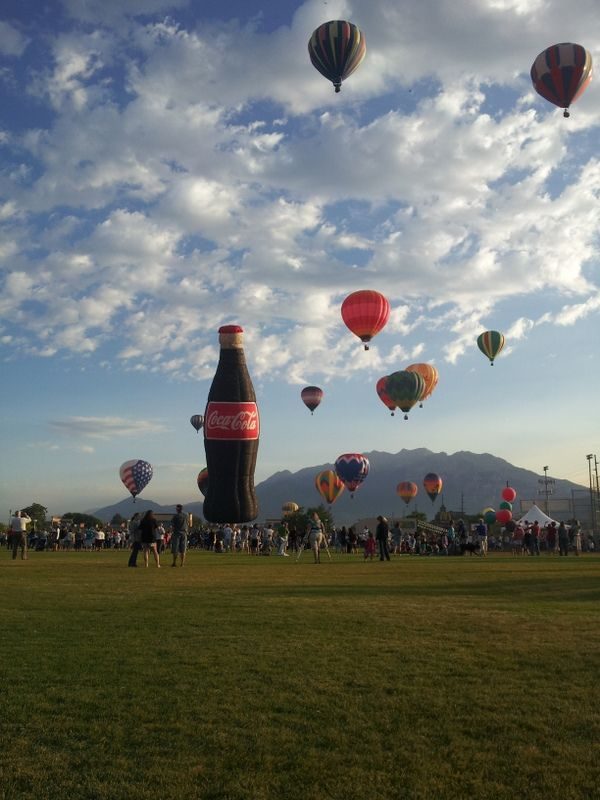
\includegraphics[width=\textwidth]{baloon_resized_color.jpg}
\caption*{original image}
\end{minipage}
\hspace{0.5cm}
\begin{minipage}[b]{0.45\linewidth}
\centering
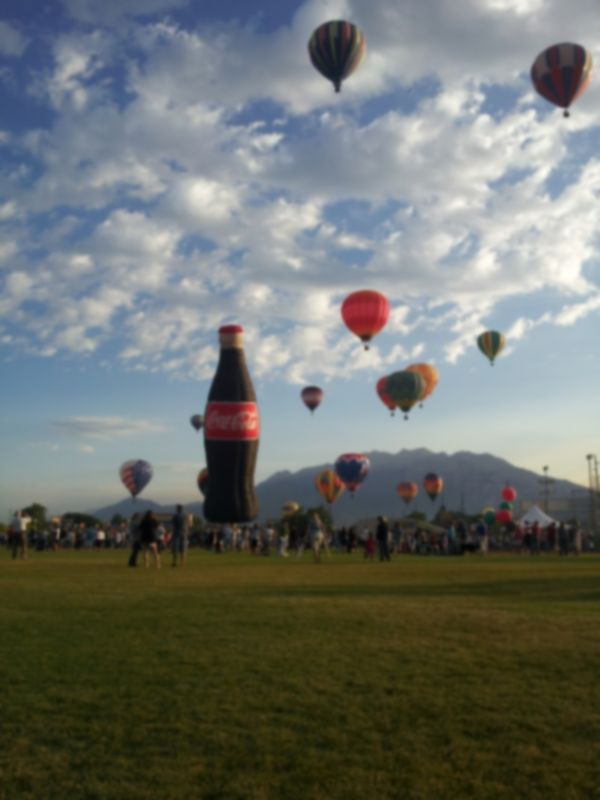
\includegraphics[width=\textwidth]{baloon_resized_color_5.jpg}
\caption*{after 5 iterations with $\sigma = .7$ and $\lambda = .2$}
\end{minipage}
\begin{minipage}[b]{0.45\linewidth}
\centering
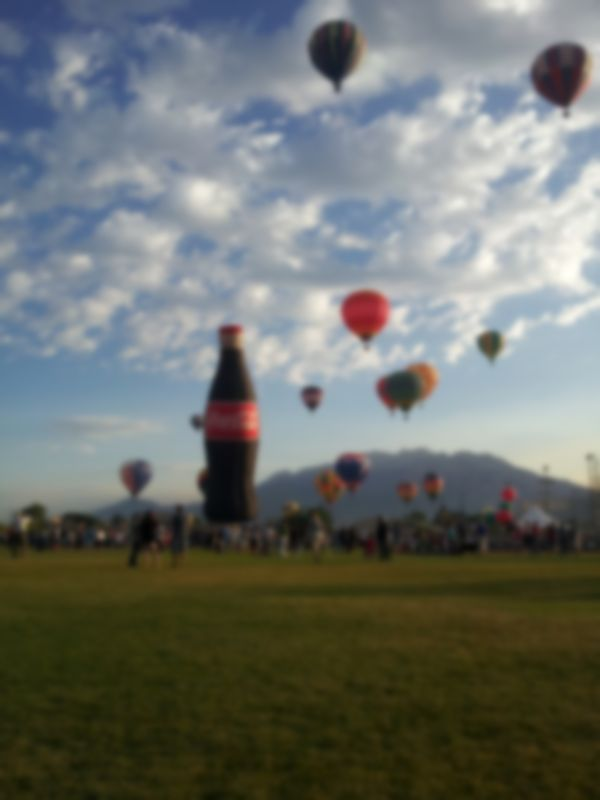
\includegraphics[width=\textwidth]{baloon_resized_color_20.jpg}
\caption*{after 20 iterations}
\end{minipage}
\hspace{0.5cm}
\begin{minipage}[b]{0.45\linewidth}
\centering
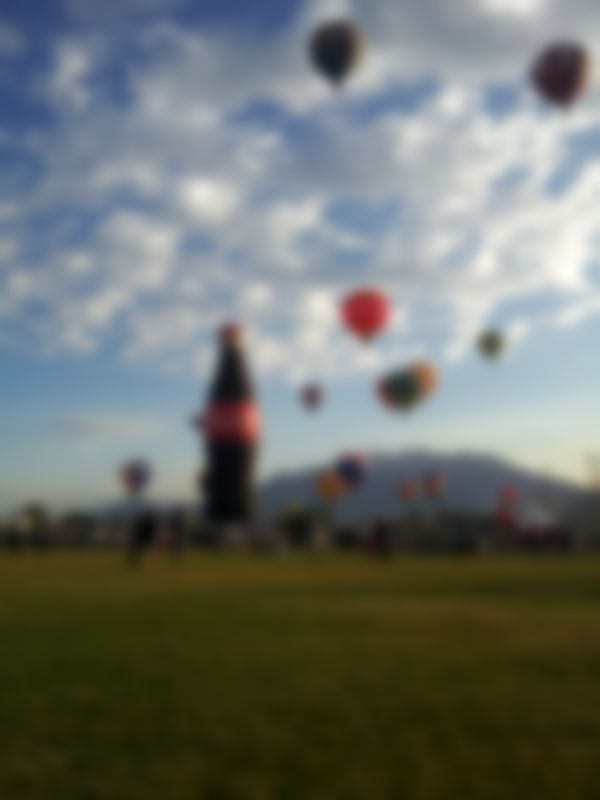
\includegraphics[width=\textwidth]{baloon_resized_color_100.jpg}
\caption*{after 100 iterations}
\end{minipage}
\end{figure}
\vfill
\clearpage

Colored images can be processed in a similar manner.
Instead of being represented as a two-dimensional array, colored images are represented as three dimensional arrays.
The third dimension is used to store the intensities of each of the standard 3 colors.
This diffusion process can be carried out in the exact same way, on each of the arrays of intensities for each color, but instead of detecting edges just in one color, we need to detect edges in any color, so instead of using something of the form $g(|U_{l+1,m}^n - U_{l,m}^n|)$ as before, we will now use something of the form $g(||U_{l+1,m}^n - U_{l,m}^n||)$, where $U_{l+1,m}^n$ and $U_{l,m}^n$ are vectors now instead of scalars.
The difference scheme can be treated as an eqation on vectors in 3-space and now reads:
\begin{equation*}
\begin{split}
U_{l,m}^{n+1} =& U_{l,m}^n + \lambda (g(||U_{l-1,m}^n - U_{l,m}^n||)(U_{l-1,m}^n - U_{l,m}^n) + g(||U_{l+1,m}^n - U_{l,m}^n||)(U_{l+1,m}^n - U_{l,m}^n) \\
 &+ g(||U_{l,m-1}^n - U_{l,m}^n||)(U_{l,m-1}^n - U_{l,m}^n) + g(||U_{l,m+1}^n - U_{l,m}^n||)(U_{l,m+1}^n - U_{l,m}^n))
\end{split}
\end{equation*}

When implementing this scheme for colored images, use the infinity norm on 3-space, i.e $||x||=max(x1,x2,x3)$ where $x1$, $x2$, and $x3$ are the different coordinates of $x$.

\begin{problem}
Make a new version of the code you wrote for the previous problem which processes a colored image.
Measure the difference between using pixels using the infinity norm.
Do not treat the colors of each pixel separately.
\end{problem}

This sort of anisotropic diffusion can be very effective, but, depending on the image, it may also smear out edges that do not have large differences between them.
An example of this limitation can be seen in the following image.
The following are the original image and the filtered images after 20, and 100 iterations.
In this case we used $\sigma = .1$ and $\lambda = .2$

\begin{figure}[ht]
\begin{minipage}[b]{.45\linewidth}
\centering
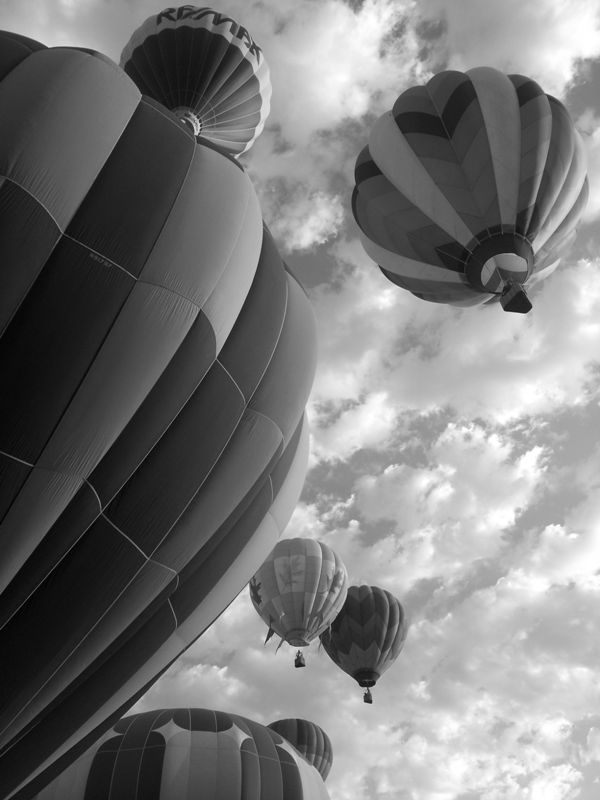
\includegraphics[width=\textwidth]{baloons_resized_bw.jpg}
\caption*{original image}
\end{minipage}
\hspace{0.5cm}
\begin{minipage}[b]{0.45\linewidth}
\centering
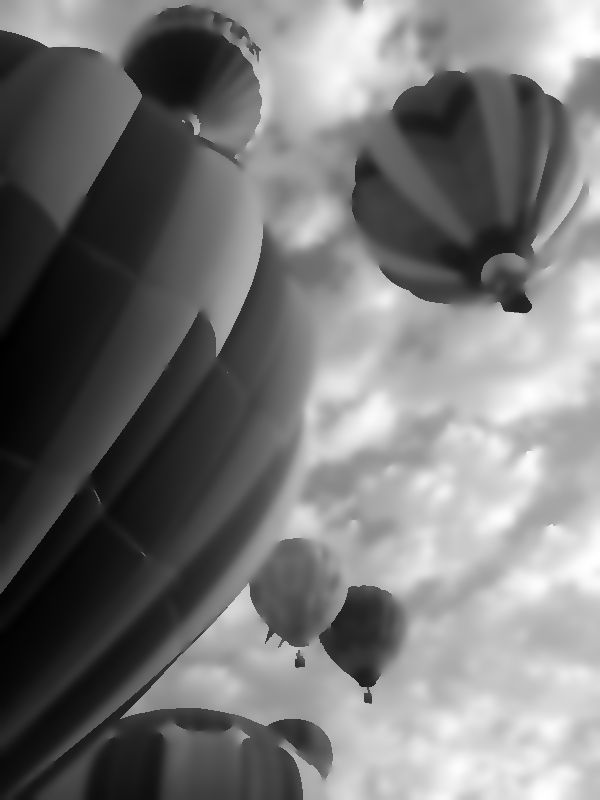
\includegraphics[width=\textwidth]{baloons_resized_bw_50.jpg}
\caption*{after 50 iterations}
\end{minipage}
\end{figure}

As we can see, after 100 iterations, some of the boundaries between similar shades of grey have smeared unevenly. You may still have to look closely to see it.
This can be counteracted somewhat by further decreasing the $\sigma$ value, but if we have random noise throughout the image, this will not remove it.
If we have random static in the image, we can remove this using a modified version of the filter.
Instead of measuring the rate of change in the picture in each direction, we change each point according to whether or not any of its adjacent points have roughly the same value it has. 
This is called a minimum-biased filter. 
This sort of trick is especially good for removing isolated pixels that are different from those around them.
A very simple way to do this is by taking the average of the two smallest differences between each pixel and its eight neighbors and using that in place of $g$ in the difference scheme above.
Along the boundaries, we do not have 8 neighbors for each pixel, but we can get by by just using the pixels we have and eliminating the other terms in the difference scheme, just as we did before.
This will make it so that points that neighbor points of similar value will not be changed, while points that do not match their surroundings will be faded to become more like the points surrounding them.
This does not have the same symmetrical diffusion as the other scheme, i.e. if one pixel changes, it does not necessarily change its neighboring pixels by the same amount.
As long as you leave $\lambda \leq \frac{1}{4}$ and you have scaled the pixels to have floating point values between 0 and 1, the scheme will still remain within its minimum and maximum bounds, since the tendency is always to move points closer to the values of their neighbors.
To demonstrate the action of such a filter, we make changes to random pixels in the color version of the same photo and use both filters to remove the noise we have added.
Below, we include an example where we have added noise to the color version of that same picture, then used a minimum-biased filter to diminish the noise and the original filter to smooth what remains.

\begin{problem}
Implement the minimum-biased finite difference scheme described above. 
\end{problem}

\newpage
\vfill
\begin{figure}[ht]
\begin{minipage}[b]{0.45\linewidth}
\centering
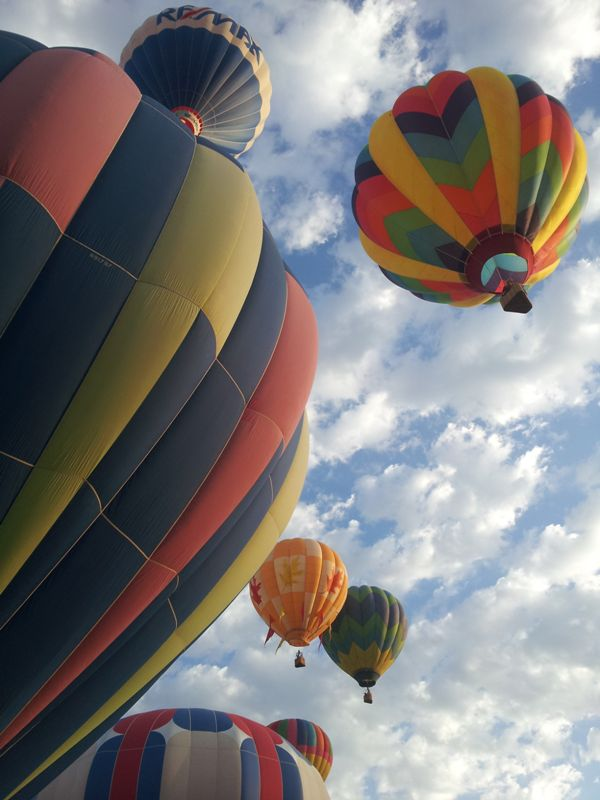
\includegraphics[width=\textwidth]{baloons_resized_color.jpg}
\caption*{original image}
\end{minipage}
\hspace{0.5cm}
\begin{minipage}[b]{0.45\linewidth}
\centering
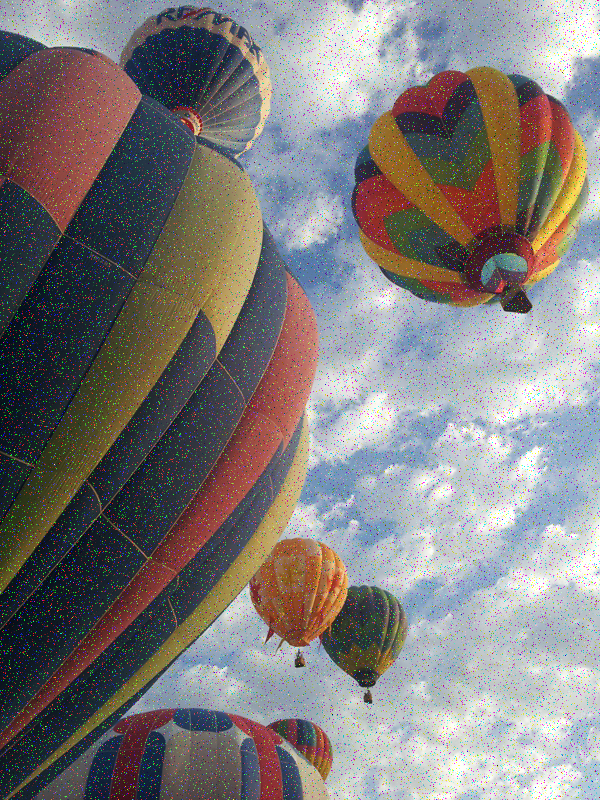
\includegraphics[width=\textwidth]{baloons_resized_noisy.png}
\caption*{randomly changed 100000 color values}
\end{minipage}
\begin{minipage}[b]{0.45\linewidth}
\centering
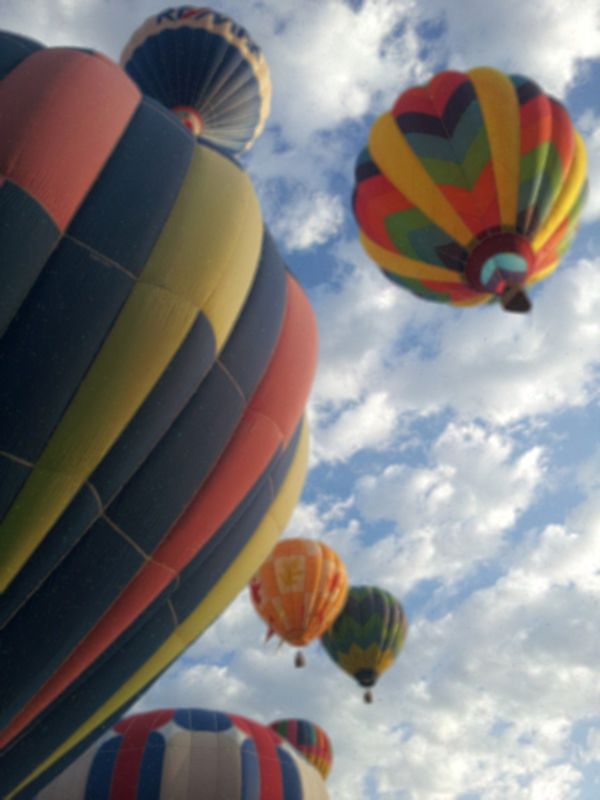
\includegraphics[width=\textwidth]{baloons_resized_minbias.jpg}
\caption*{300 iterations of a min-biased scheme}
\end{minipage}
\hspace{0.5cm}
\begin{minipage}[b]{0.45\linewidth}
\centering
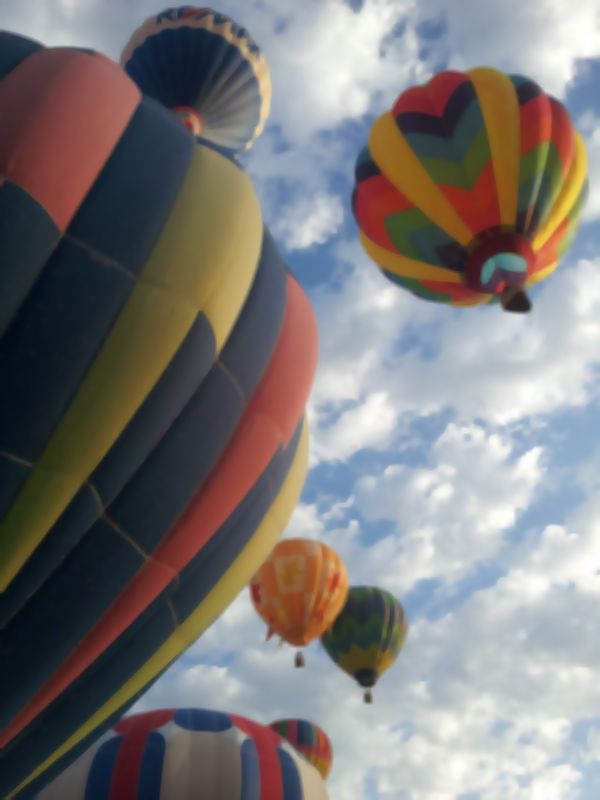
\includegraphics[width=\textwidth]{baloons_resized_both.jpg}
\caption*{after 8 additional iterations of the first filter with $\lambda=.25$ and $\sigma=.04$.}
\end{minipage}
\end{figure}
\vfill
\clearpage

\nocite{Perona1988,Kim2009}
\printbibliography